\documentclass[12pt]{article}

% Solutions toggle
\newif\ifsolutions
\solutionsfalse
%% \solutionstrue

% ASSIGNMENT NUMBER
\newcommand{\hwnumber}{4}
\newcommand{\booksection}{}
\newcommand{\duedate}{}
% -------------

%%% Packages
\usepackage[margin=1in, footskip=24pt, headheight=24pt]{geometry}
\usepackage{amsmath, amssymb, amsthm, graphicx}
\usepackage{mathtools}
\DeclarePairedDelimiter\ceil{\lceil}{\rceil}
\DeclarePairedDelimiter\floor{\lfloor}{\rfloor}
\usepackage[colorlinks, urlcolor=blue]{hyperref}
\usepackage{color}
\usepackage{comment}
\usepackage{enumerate}
\usepackage{lastpage}
\usepackage{multirow, multicol}
\usepackage{tikz}
\usetikzlibrary{matrix,decorations.text,decorations.pathmorphing,decorations.markings,arrows,calc,shapes.geometric,patterns,shadows,intersections,decorations.markings,decorations.pathreplacing,decorations.pathreplacing,backgrounds,angles,quotes}
\usepackage{pgfplots}
\pgfplotsset{compat=1.16}

\usepackage{fancyhdr}

\pagestyle{fancy}
%% \renewcommand{\familydefault}{\sfdefault}

\newcommand{\R}{\mathbb{R}}
\newcommand{\ddx}{\frac{d}{dx}}

\global\long\def\V#1{\boldsymbol{#1}} %vector
\global\long\def\M#1{\boldsymbol{#1}} %matrix

\global\long\def\D#1{\Delta#1} %\D{t} for time step size
\global\long\def\d#1{\delta#1} %\d{t} for small increment

\global\long\def\norm#1{\left\Vert #1\right\Vert }
\global\long\def\abs#1{\left|#1\right|}

\global\long\def\grad{\M{\nabla}}
\global\long\def\av#1{\left\langle #1\right\rangle }

% HEADER MACROS
\newcommand{\term}{Spring 2022 \& 2023}
\newcommand{\coursename}{Intro Math Modeling}
\newcommand{\coursenumber}{MATH-UA 251}
\newcommand{\course}{\coursename \ (\coursenumber)}

\fancyhead[RO]{\term}
\fancyhead[LO]{\course}
% -------------

%%% Theorem Styles
\theoremstyle{definition}
\newtheorem{ex}{Exercise}

%%%%%%%%%%%%%%%%%%%%%%%% Solutions %%%%%%%%%%%%%%%%%%%%%%%%%%%%%
% \begin{solution} and \begin{answerspace} must be at the beginning of the line.
% Doesn't work inside the \myversions command. Use if statements instead.
% No underscores in comment names

\ifsolutions
\newenvironment{solution}{\color{blue}}{} \excludecomment{answerspace} \newenvironment{notes}{\color{red} \noindent Grading Notes:}{}
\else
\excludecomment{notes} \excludecomment{solution} \includecomment{answerspace} 
\fi
%%%%%%%%%%%%%%%%%%%% End Solutions %%%%%%%%%%%%%%%%%%%%%%%e}


\begin{document}
% HEADER
\begin{center}
%% \ifsolutions
%%   \textbf{\Large Homework \hwnumber\ - \booksection\ (Solutions)}\\
%% \else
%%   \textbf{\Large Homework \hwnumber\ - \booksection}\\
%% \fi
\ifsolutions
  \textbf{\Large Homework \hwnumber\ (Solutions)}\\
\else
  \textbf{\Large Homework \hwnumber}\\
\fi
\vspace{12pt}
Due date: someday, sometime! \duedate

Submit on NYU Brightspace.
\end{center}

%% \noindent Please give complete, well-written solutions to the following exercise. Provide sufficient justification and explanation for a classmate who has not worked on the exercise to understand your solution.


\begin{ex}
  
  [100 pts] Fruits on trees can freeze in Winter time even when the ambient temperature is above $0\;\mathrm{^oC}$. This exercise tries to explain this counterintuitive phenomenon.

  Consider a spherical-shape orange of radius $a$ in an ambient with temperature $T_{\infty}$ and heat transfer coefficient $h$. The orange also radiates, with emissivity $\epsilon$, to the sky with an effective temperature $T_s$. Assume a spatially uniform temperature within and on the surface of the orange.
  
  \begin{enumerate}[(i)]\setlength{\itemsep}{0pt}
  \item Write an energy balance for the orange taking into account the convection to the ambient and radiation to the sky (neglect radiation to the ambient). Simplify the equation for constant $\rho$ and $C_p$ of the orange, to reach to an ordinary differential equation (ODE) for the temperature of the orange, $T$, as a function of time $t$.
  \item Use Euler's method to solve the ODE. Assume that the physical properties of orange are close to those of water, i.e., $\rho=1000\;\mathrm{kg/m^3},\;C_p=4184\;\mathrm{J/(kg\cdot K)}$. Let $T_{\infty}=2\;\mathrm{^oC},\;h=20\;\mathrm{W/(m^2\cdot K)}\;a=5\;\mathrm{cm},\;\epsilon=1$. Consider three different effective sky temperatures $-20,-10,-5\;\mathrm{^oC}$. (Careful! The radiation equation works with absolute temperature in $\mathrm{K}$ not $\mathrm{^oC}$.) Make a plot of the orange temperature $T$ in Celsius ($\mathrm{^oC}$) versus time in minutes for each sky temperature. Also, plot horizontal black (different from the other three curves) lines at $T=0\;\mathrm{^oC}$ and $T=T_{\infty}$ to denote the freezing and ambient temperatures. Use an initial temperature $10\;\mathrm{^oC}$ and simulate each problem for $7\tau$, where $\tau=mC_p/(hA)$ is the convection time scale. Also, use $\Delta t=0.01\tau$. For each of the sky temperatures, you should see that the orange temperature reaches to a constant, equilibrium (or steady-state), value (not changing significantly with time). If this constant value is below the freezing temperature, the orange freezes! Does this happen here for any of the sky temperatures?
  \item The steady-state value can be obtained directly from the ODE by using the Newton's method. Find the steady-state temperature for the three cases above directly, and compare to the values you obtained by time marching in item (ii). With the latter, take the last calculated temperature as the equilibrium temperature.
  \item In a separate figure, plot the sky temperature required for a $0\;\mathrm{^oC}$ ($273.15\;\mathrm{K}$) equilibrium temperature as a function of $0\le T_{\infty}\;(\mathrm{^oC})\le10$. Next, explain, mathematically, under what conditions (for what $T_{\infty}$), there is no Real valued $T_s$. What does it mean physically?
  \end{enumerate}
\noindent\textbf{\textcolor{red}{notes:} }You need to submit your \textbf{CODE} (commented) as well. Also, include your \textbf{PLOTs} in the report. As a general rule, any results obtained by the code (whether it is a plot or a computed value) should be included in the report. Solutions without interpretation of the results will not receive full credits.

\begin{solution}
  The balance equation can be expressed as
  $$\frac{d(mC_pT)}{dt}=-hA(T-T_{\infty})-\sigma\epsilon A(T^4-T_s^4),$$
  where $m$ is the mass of the orange, $A=4\pi a^2$ is its outer surface area, and $\sigma=5.7\times10^{-8}\;\mathrm{W/(m^2\cdot K^4)}$ is the Stefan-Boltzmann constant. For constant $\rho$ (or $m$ since the orange volume is constant) and $C_p$, the above ODE simplifies to
  $$\frac{dT}{dt}=-\frac{hA}{mC_p}(T-T_{\infty})-\frac{\sigma\epsilon A}{mC_p}\left(T^4-T_s^4\right).$$
  Using Euler's method:
  $$T_{i+1}=T_i-\Delta t\left[\frac{hA}{mC_p}(T_i-T_{\infty})+\frac{\sigma\epsilon A}{mC_p}\left(T_i^4-T_s^4\right)\right],$$
  where $i=0,1,2,\dots$ denotes the time step. The figure below shows the simulation results. Also see HW4\_orange.py.
  \begin{figure}[h]
  \centering
  \resizebox{0.6\textwidth}{!}{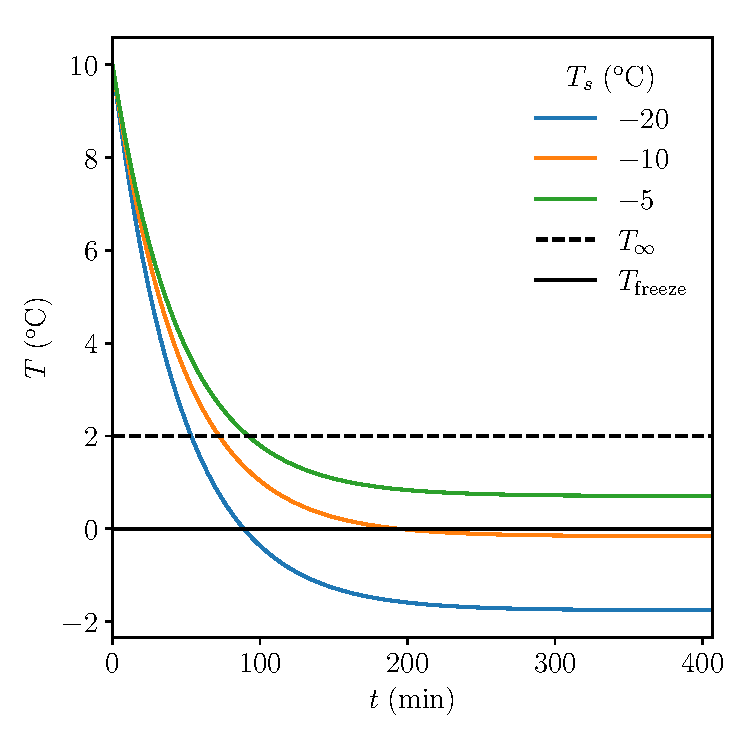
\includegraphics{orange.pdf}}
  \end{figure}

  To directly find the equilibrium temperatures, we let $dT/dt=0$, and find $T$ from the resulting algebraic equation using the Newton's method:
  $$f=h(T-T_{\infty})+\sigma\epsilon(T^4-T_s^4)=0\Rightarrow f'=h+4\sigma\epsilon T^3\Rightarrow T_{k+1}=T_k-\frac{f}{f'}.$$
  Again see HW4\_orange.py for details of implementation. Table below summarizes the equilibrium temperatures in $\mathrm{^oC}$ for different cases. For the Newton's method, a tolerance of $|f(T_k)|<10^{-7}$ was used.
  \begin{center}
    \begin{tabular}{ c | c  c }
      $T_s\;\mathrm{^oC}$ & Newton & Euler\\
      \hline
      $-20$ & $-1.7565$ & $-1.7545$ \\
      $-10$ & $-0.1614$ & $-0.1596$ \\
      $-5$  & $0.7053$ & $0.7069$ \\
    \end{tabular}
\end{center}

  To find the required $T_s$ for a given $T_{\infty}$, we substitute $T=273.15\;\mathrm{K}$ in the steady-state equation above:
  $$f=h(273.15-T_{\infty})+\sigma\epsilon(273.15^4-T_s^4)=0\Rightarrow T_s=\left[\frac{h}{\sigma\epsilon}(273.15-T_{\infty})+273.15^4\right]^{\tfrac{1}{4}}.$$
  Figure below shows a plot of $T_s$ versus $T_{\infty}$ using the obtained equation. Note that for $T_{\infty}=0\;\mathrm{^oC}$, we get $T_s=0\;\mathrm{^oC}$. Also, note that if the expression in the brackets is negative, $T_s$ will be a complex number. So the minimum possible value for the expression is $0$ which occurs for
  $$T_{\infty}^{\mathrm{critical}}=273.15+\frac{\sigma\epsilon}{h}273.15^4=289.0153\;\mathrm{K}=15.8653\;\mathrm{^oC}.$$
  At this critical $T_{\infty}$, the required sky temperature becomes $0\;\mathrm{K}$ (absolute zero!). We can't go beyond that!
  \begin{figure}[h]
  \centering
  \resizebox{0.6\textwidth}{!}{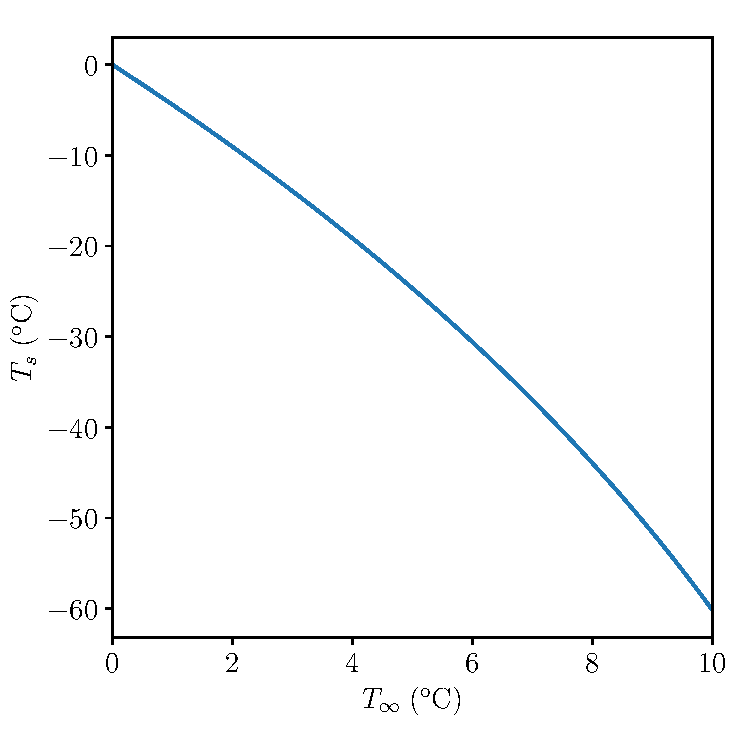
\includegraphics{Ts_VS_Tinf.pdf}}
  \end{figure}
  
\end{solution}
\end{ex}


\end{document}
